\documentclass[]{iac}
% To make the list of abbreviations and symbols.
\usepackage[acronym]{glossaries}
\makeglossaries
% This packagae is used to make list of symbols and list of abbreviations at the start of the report. 
% \makeglossaries
% This is the syntax for the symbol 
% \newglossaryentry{here comes the command you will use}
% {
%         name=here comes the symbol,
%         description={Is a mark up language specially suited for 
% scientific documents}
% }
% This is the syntax for abbreviations 
% \newacronym{here comes the command you will use}{here comes the abbereviation}{here comes the full form of the abbreviation}

% These are the commands to be used in the text:
% For the symbol  
% \gls{here comes the command you will use} -->  first letter small 
% \Gls{here comes the command you will use} -->  first letter caps
% \glspl{here comes the command you will use} -->  first letter small and plural 
% \Glspl{here comes the command you will use} -->  first letter caps and plural 

% For the abbreviations: 
% \acrshort{here comes the command you will use} -> will use the abbreviation 
% \acrlong{here comes the command you will use} -> will use the full form 
% \acrfull{here comes the command you will use} -> will use the full form (abbreviation).  

\newacronym{test}{TEST}{This section is not numbered. A nomenclature section could be provided when there are mathematical symbols in your paper. Superscripts and subscripts must be listed separately. Nomenclature definitions should not appear again in the text.
}
\newacronym{iac}{IAC}{This section is not numbered. A nomenclature section could be provided when there are mathematical symbols in your paper. Superscripts and subscripts must be listed separately. Nomenclature definitions should not appear again in the text.
}

\newglossaryentry{test_symbol}
{
        name=$\theta_{test}$, 
        description={This section is not numbered. Define acronyms and abbreviations that are not standard in this section. Such acronyms and abbreviations that are unavoidable in the abstract must be defined at their first mention there. Ensure consistency of abbreviations throughout the article. Always use the full title followed by the acronym (abbreviation) to be used, e.g., reusable suborbital launch vehicle (RSLV), International Space Station (ISS).}
}

\DeclareMathOperator{\E}{E}
\DeclareMathOperator{\prob}{p}
\DeclareMathOperator{\tr}{tr}

\newcommand{\etalia}{\textit{et al.}}
\newcommand*{\vectornorm}[1]{\left\|#1\right\|}
\newcommand*\rfrac[2]{{{}^{#1}\!/_{#2}}} % running fraction with slash - requires math mode.
\newcommand*\T{\mathsf{T}}

\begin{document}

\IACpaperyear{20}
\IACpapernumber{D9.2.8}
\IACconference{71}
\IAClocation{The CyberSpace Edition, 12-14 October 2020}
\IACcopyrightA{2020}{International Astronautical Federation (IAF)}

\title{Manuscript Template and Style Guide (Title of your paper)}

\IACauthor{Main-Author\textsuperscript{a}*,}{\textsuperscript{a} \emph{Department of Tourism and Hospitality, China
    University of Science and Technology, 200 Chunghwa Street, Henshan
    Village, Hsinchu County, Taiwan 31241}, \emph{\uline{eva77tw@cc.hc.cust.edu.tw}}}

\IACauthor{Co-Author}{\textsuperscript{b} \emph{Department of Aerospace Engineering, Ryerson University, 350 Victoria Street, Toronto, Ontario, Canada M5B 2K3},
\emph{\uline{editor-in-chief@iaamail.org}}}


\abstract{~~~~A concise and factual abstract (written in third person and in one paragraph) of no more than 400 words is required. The abstract should state briefly the purpose of the research, the principal results and major conclusions. An abstract must be stand alone and complete in itself with no references to the main body of the manuscript. References should be avoided, but if essential, then cite the author(s) and year(s). Also, non-standard or uncommon abbreviations should be avoided, but if essential they must be defined at their first mention in the abstract itself. Readers should not have to read the full text to understand the abstract. The abstract can be an updated version of the one submitted at the call-for-abstracts, but its contents must not differ substantially.}

\IACkeywords{maximum 6 keywords}{}{}{}{}{}

\maketitle
% Add list of symbols
\printglossary[type=\acronymtype, title=Abbreviations]
\printglossary[title=Nomenclature]

\section{Introductions}
Section headings are in bold and placed flush on the left hand margin of the column.

The Introduction Section is to state the objectives of the work, provide an adequate background including a brief literature survey, major differences from the others, and sectional organization of this paper. Avoid a too detailed and lengthy literature survey and a summary of the results.

Divide your paper into clearly defined and numbered sections numbered 1., 2., …. Subsections should be numbered 1.1 (then 1.1.1, 1.1.2, ...), 1.2, etc. Use this numbering also for internal cross-referencing: do not just refer to “the text”. Any subsection may be given a brief heading. Each heading should appear on its own separate line.

\subsection{Subheadings}
Subheadings are underlined and placed flush on the left-hand margin of the column.

\subsubsection{Sub-subheadings}
Sub-subheadings are underlined and indented.

\section{Materials and methods}
Provide sufficient detail to allow the work to be reproduced. Methods already published should be indicated by a reference: only relevant modifications should be described.

\section{Theory and calculation}
A Theory section should extend, not repeat, the background to the article already dealt with in the Introduction and lay the foundation for further work. In contrast, a Calculation section represents a practical development from a theoretical basis.

\subsection{Equation Numbers}
When numbering equations, enclose numbers in brackets and place flush right with the right-hand margin of the column. The numbers identifying the equations should be placed in parentheses to the right of the equation. For example:

\begin{equation}
\stackrel{\star}{F}_{12} = -G \cdot \frac{ m_1 \cdot m_2 }{ \left\|\stackrel{\star}{r}_2 - \stackrel{\star}{r}_1\right\|^2 } \cdot \hat{u}_{12}
\end{equation}

\subsection{Illustrations and Captions}
It is important to remember that all artwork, captions, figures (\textit{e.g.}, Fig.~\ref{fig:X}), graphs, and tables (such as Table~\ref{table:X}) will be reproduced exactly as you submitted them. (\textbf{Company logos} and \textbf{identification numbers} are not permitted on your illustrations.)

\begin{figure}
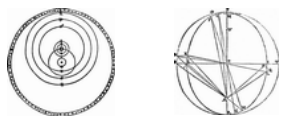
\includegraphics[width=\columnwidth]{examplefigure.png}
\caption{\label{fig:X}Title of the figure, left-justified, subsequent text indented. Place figures at the top or bottom of a column wherever possible, as close as possible to the first references to them in the manuscript. Restrict them to single-column width unless this would make them illegible.}
\end{figure}

\subsection{Graph Lines, Drawings, and Tables}
Use black ink on white manuscript and position to fit within one of the columns on the page, and ensure that they remain still readable.

Tables with a moderate amount of information should be positioned within one column. Tables, graphs, or pictures with large amounts of information may extend across two columns.

\begin{table}
\begin{tabular}{rllll}
\toprule
& Venus & Earth & Mars & Jupiter \\
\midrule
$\rfrac{M}{M_E}$	& 0.82 		& 1 		& 0.11 		& 317.89	\\
$e$					& 0.007		& 0.017		& 0.093		& 0.048		\\
$R$ (AU)			& 0.7233	& 1			& 1.524		& 5.203		\\
$i$ (deg)			& 3.40		& 0			& 1.85		& 1.30		\\
$T$ (years)			& 0.62		& 1			& 1.88		& 11.86		\\
\bottomrule
\end{tabular}
\caption{\label{table:X}Title of table, left justified, subsequent text indented. Heading centered. Do not use vertical lines within the table; use horizontal lines only to separate headings from table entries.}
\end{table}

\section{Style Guide}

\subsection{Acronyms}
Always use the full title followed by the acronym to be used \acrfull{test}.

\subsection{Symbols}
Test the symbol \gls{test_symbol}

\subsection{References}
List and number all the bibliographical references at the end of the full text, in the order of appearance.\cite{Geim2001}

\subsection{Captions, Graph Axes, Legends}
Captions, graph axes, legends, \textit{etc.}, should be large enough to remain legible.

\subsection{Footnotes, Symbols, and Abbreviations}
Footnotes should be cited using symbols in this order: \footnote{Footnote 1} \footnote{Footnote 2} \footnote{Footnote 3} \footnote{Footnote 4} \footnote{Footnote 5} \footnote{Footnote 6} \footnote{Footnote 7} \footnote{Footnote 8}. Use only standard symbols and abbreviations in text and illustrations.

\subsection{Page Numbers}
Indicate page numbering at the bottom of each page.

\bibliographystyle{plain}
\bibliography{example}

\end{document}